%%%%%%%%%%%%%%%%%%%%%%%%%%%%%%%%%%%%%%%%%%%%%%%%%%%%%%%%%%%%%%
\section{Introdução}


%%%%%%%%%%%%%%%%%%%%%%%%%%
\begin{frame}
\frametitle{Introdução}
\begin{minipage}{0.47\textwidth}
    \begin{itemize}
        \item Histórico
        \item Contexto
        \item Exemplo: \textit{Alo Mundo}
        \item Como usar
    \end{itemize}
\end{minipage}
\begin{minipage}{0.5\textwidth}
\begin{figure}[ht!]
\begin{center}
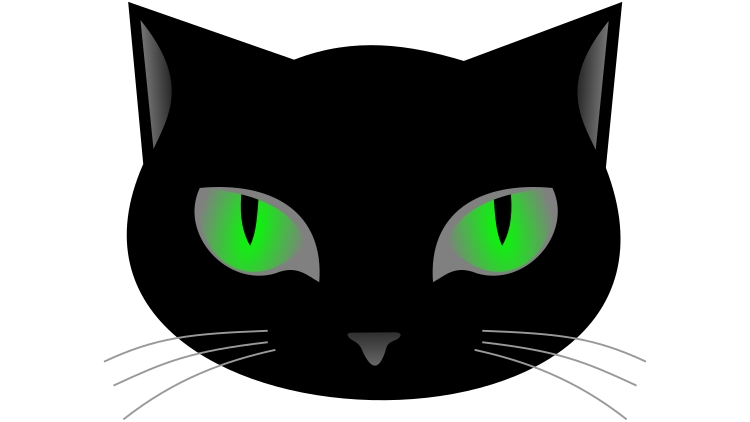
\includegraphics[width=1.2\textwidth, height=0.40\textheight]{figures/logo_picat_alex.jpg}
\end{center}
\end{figure}
\end{minipage}
\end{frame}
%%%%%%%%%%%%%%%%%%%%%%%%%%


\subsection{Histórico}

\begin{frame}

    \frametitle{Histórico}

    \begin{itemize}
      \item Criada em 2013 por Neng-Fa Zhou e Jonathan Fruhman -- USA

      \item Utiliza o B-Prolog (Neng-Fa Zhou) como base de implementação, tendo
      a Lógica de Primeira-Ordem (LPO) como parte de seu mecanismo programação

\pause
      \item Uma evolução ao Prolog após seus mais de 40 anos de sucesso!

\pause
      \item Sua atual versão é a 2.x (\today).
\pause
      \item Código-aberto, segue as regras da FSF

    \end{itemize}
\end{frame}

%%%%%%%%%%%%%%%%%%%%%%%%%%%%%%%%%%%%%%%%%%%%%%%%%%%%%%%%%%%%%%%%%%%%%

\subsection{\textit{Links Iniciais}}
\begin{frame}[fragile]
  \frametitle{Links do PICAT}

  \begin{itemize}
   	\item Site oficial: \textbf{\textcolor{violet}{\url{http://picat-lang.org}}} -- links, forum, livro, videos etc

   	\item Site do Hakan -- Suécia:  \url{http://www.hakank.org/picat/}

  \item   \textbf{Videoaula 01: Introdução ao PICAT}, disponível no Youtube:\\
    \textbf{\url {https://www.youtube.com/watch?v=0DmTyFFQPK8}}

   \item   \textbf{Videoaula 02: Introdução ao PICAT}, disponível no Youtube:\\
  \textbf{\url {https://www.youtube.com/watch?v=7fPKPd0ZDnc}}

   \item   \textbf{Videoaula: Depuração com PICAT}, disponível no Youtube:\\
  \textbf{\url {https://www.youtube.com/watch?v=9axovyzMqwc}}

    
   	\item Editor on-line mantido pelo Alexandre: \url{http://retina.inf.ufsc.br/picat.html}
     
    
    \item Se não tiver \textit{plugin} para Picat, escolha a sintaxe da linguagem \textit{Erlang}.
    
  \end{itemize}

\end{frame}

%%%%%%%%%%%%%%%%%%%%%%%%%%%%%%%%%%%%%%%%%%%%%%%%%%%%%%%%%%%%%%%%%%%%%

\subsection{Estrutura da Linguagem}

\begin{frame}
	\frametitle{Conhecendo PICAT}
    
    \begin{itemize}
    
    	\item Picat é uma linguagem de programação simples de usar, poderosa e multi-uso
        
        \item Alguma de suas características 
         são associadas com linguagens lógicas, como Prolog, B-Prolog, Goedel, etc
        
        \pause
        \item Picat é uma linguagem essencialmente \underline{\textbf{multiparadigma}},
        abrangendo partes de vários paradigmas de programação: \underline{declarativo} (lógico e funcional) e    \underline{ imperativo}
        
        %\item Esta combinação de características declarativas e imperativas permite
        %o desenvolvimento de softwares mais produtivos, mas que ainda possam ser altamente 
        %otimizados para tarefas específicas, ou softwares mais simples para tarefas mais mundanas;
        
    \end{itemize}
    
\end{frame}

%%%%%%%%%%%%%%%%%%%%%%%%%%%%%%%%%%%%%%%%%%%%%%%%%%%%%%%%%%%%%%%%%%%%%

\subsection{Multiparadigma}
\begin{frame}[fragile]
    \frametitle{O que é ser Multiparadigma ?}

    \begin{itemize}
    
    \item Paradigma: um conjunto de características baseado em alguma abordagem teórica 
    
    \pause
      \item Picat é uma linguagem multiparadigma pois abrange os seguintes paradigmas:
    
      \begin{itemize}
      	\item[--] Lógico
      	\item[--] Funcional
      	\item[--] Procedural
      \end{itemize}
      
     \pause
      \item Em resumo,  \textit{uma boa mistura} de: Haskell (Funcional) , Prolog (Lógica) e 
      Python (Procedural e Funcional).
      
    \end{itemize}
      
\textbf{\textcolor{red}{Pular .... leiam com calma, depois!}}
\end{frame}

%%%%%%%%%%%%%%%%%%%%%%%%%%%%%%%%%%%%%%%%%%%%%%%%%%%%%%%%%%%%%%%%%%%%%
\subsection{Outros Paradigmas}
\begin{frame}[fragile]
	\frametitle{Paradigma Lógico}
    
    \begin{itemize}
    
    	\item Uma linguagem lógica é uma onde o programa é expresso como um conjunto
        de predicados lógicos, escritos por \textit{fatos} e \textit{regras}
    
    \pause
    	\item Regras são escritas em formas de cláusulas, as quais são interpretadas como
        implicações lógicas.\\ 
        Dependem das premissas serem verdadeiras para esta ser verdadeira.
        

    \pause
    	\item Fatos são cláusulas sem premissas, verdades absolutas.

        
        \pause
        \item Este   paradigma é a  \textbf{base} do Picat
    \end{itemize}

\end{frame}

%%%%%%%%%%%%%%%%%%%%%%%%%%%%%%%%%%%%%%%%%%%%%%%%%%%%%%%%%%%%%%%%%%%%%

\begin{frame}[fragile]
	\frametitle{Paradigma Funcional}
    
    \begin{itemize}
    
    
    	\item Uma linguagem funcional é uma onde os elementos do programa podem ser avaliados e 
        tratados como funções matemáticas.
        
        \pause
         \item Um dos principais motivos em usar linguagens funcionais é a previsibilidade
         e facilidade no entendimento do estado atual do programa.
         
         \pause
         \item Este fato de uma  sintaxe simples, torna o Picat  intuitivo e legível na
         funcionalidade de seus códigos.
         
    \end{itemize}
    
    
\end{frame}

%%%%%%%%%%%%%%%%%%%%%%%%%%%%%%%%%%%%%%%%%%%%%%%%%%%%%%%%%%%%%%%%%%%%%

\begin{frame}[fragile]
	\frametitle{Paradigma Procedural}
    
    \begin{itemize}
    
    	\item Uma linguagem procedural é uma que pode ser subdividida em \textit{procedimentos},
        também chamados de rotinas, subrotinas ou funções
        
        \pause
        \item Em linguagens procedurais há um procedimento principal (em geral é chamado de 
        \textit{Main}) que controla o uso e a chamada de outros procedimentos. Em Picat há
        tal hierarquia.
        
        \pause
        \item Em Picat, cada premissa é tratada como um procedimento, que é resolvido por meio
        de métodos de inferência lógica.
       
    \end{itemize}
    
\framebreak
    
    \begin{figure}
    	\begin{columns}
    		\column{.6\linewidth}
	         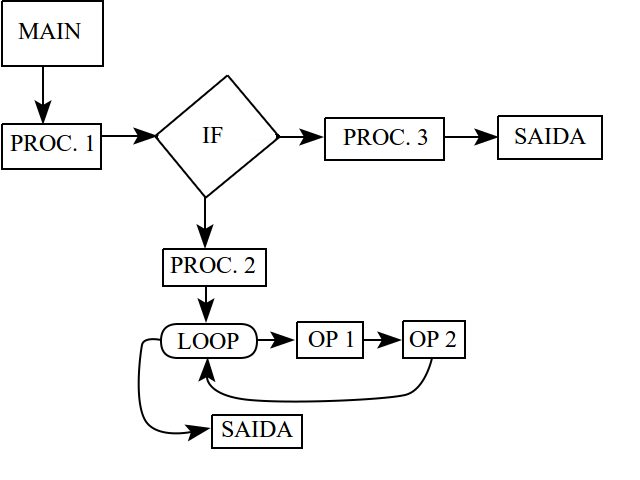
\includegraphics[width=.8\textwidth] {figures/Paradigma_Procedural.png}
             \column{.4\linewidth}
             \caption{Fluxograma representando a estrutura de um programa Procedural}
	         \label{Fluxograma Procedural}
		\end{columns}
	\end{figure}

\textbf{\textcolor{red}{Até aqui ...}}    
\end{frame}

%%%%%%%%%%%%%%%%%%%%%%%%%%%%%%%%%%%%%%%%%%%%%%%%%%%%%%%%%%%%%%%%%%%%%

\begin{frame}[fragile]
    \frametitle{Algumas Características:}

\textbf{\textcolor{red}{Retornar aqui ....}}
    \begin{itemize}
    
    \pause 
      \item Sintaxe elegante e simples, facilitando a leitura e entendimento do código
      
          \pause 
      \item Velocidade de execução em um ambiente \textit{interpretado} (há
      uma \textit{máquina   virtual} como Python, Java e alguns Prologs)
      
          \pause 
      \item Disponibilidade em vários sistemas operacionais e arquiteturas
      
      \pause 
      \item Análogo a Python, podem ser feitas \textit{queries}
      ou \textit{consultas} ao terminal de Picat.

      \pause 
      \item Há várias bibliotecas da própria linguagem, e diversas ferramentas
      externas permitindo o incremento do poder do Picat.
      
    \end{itemize}
\end{frame}

%%%%%%%%%%%%%%%%%%%%%%%%%%%%%%%%%%%%%%%%%%%%%%%%%%%%%%%%%%%%%%%%%%%%%
\subsection{Comparativo com Outras Linguagens}

\begin{frame}[fragile]
	\frametitle{Comparativo com Outras Linguagens}
	
	
	\begin{itemize}

	\item Muitos conceitos herdados do Prolog (criado em 1969 e largamente utilizado em muitos projeto)
	\item Como Picat teve origem no B-Prolog, sintaxe, backtracking, ..., muitas semelhanças
	\pause
	\item Variáveis: letras Maiúsculas
	\item Átomos, predicados, functores ....: letras minúsculas
   \item  Algumas estruturas sofisticas construídas a partir de listas: mapas, filtros, dicionários, etc
   \item Código eficiente
	\pause
	
   \item Detalhe: comunidade do Prolog, enorme, já a do Picat, centenas (?)
   \item {\bf \textcolor{red}{Quanto as outras linguagens de outros paradigmas?}}

      
\end{itemize}
\end{frame}


\begin{frame}[fragile]
	\frametitle{Picat $\times$ Haskell  -- cortesia do Neng-Fa}

\vspace{-0.5 cm}
%\begin{flushleft}

%\begin{table}
	%	\begin{center}
		%	\caption{\label{tab:tab1}Picat compared to Haskell}
    \begin{scriptsize}
	\hspace*{-9 mm}\begin{tabular}{|l|l|l|} \cline{1-3}
					& \ \ \ \ \ \ \ \ \ \ \ \ \ \ \ {\bf Picat} &  \ \ \ \ \ \ \ \ \ \ \ \ \ \ \ {\bf Haskell} \\ \cline{1-3}
					Variables & logic \& dynamic & single-assignment \& static \\
					Numbers & \texttt{1},\  \texttt{0b11},\  \texttt{0o77},\  \texttt{0xff},\  \texttt{1.0},\  \texttt{1.0e10} & \texttt{1},\  \texttt{0o77},\  \texttt{0xff},\  \texttt{1.0},\  \texttt{1.0e10}\\
					Atoms   & \texttt{abc},\  \texttt{'A'},\  \texttt{'123'} & n/a \\
					Lists   & \texttt{[1,2,3]},\ \texttt{new\_list(10)} & \texttt{[1,2,3]}\\
					\ \ \ (add first) &  \texttt{L = [a$|$L0]} & \texttt{lst = ('a':lst0)}\\
					\ \ \ (add last) &  \texttt{L = [a$|$L1]},\ \texttt{L1 = [b$|$L2]} & n/a \\
					\ \ \ (index) & \texttt{L[3]}  & \texttt{lst!!2}\\
					\ \ \ (slice) & \texttt{L[2..3]}  & take 2 \$ drop 1 \$ lst \\
					\ \ \ (concatenate) & \texttt{L1++L2}  &  \texttt{lst1++lst2}\\    
					\ \ \ (comprehension) &  \texttt{[X : X in 0..10,\  even(X)]} & \texttt{[x $|$ x $<$- [0..10],\  (even x)]} \\
					\ \ \ (pattern-matching) & \texttt{L = [H$|$T]}  & \texttt{(h:t) = lst}\\
					Ranges  & \texttt{1..10},\ \texttt{10..-1..1} & \texttt{[1..10]},\ \texttt{[10,9..1]} \\
					Strings & \texttt{"abc" = [a,b,c]} & \texttt{"abc" = ['a','b','c']} \\
					Tuples & \texttt{\{a,1,[]\}} & \texttt{(a,1,[])}\\
					Hashtables   & \texttt{new\_map([a=1,\ b=2])} & \texttt{Data.HashTable} \\
					Unification   & \texttt{[X,b] = [a,Y]} & n/a\\
					Backtracking   & \texttt{member(X,\ [a,b,c])} & n/a \\ \cline{1-3}        
				\end{tabular}
			\end{scriptsize}
	%	\end{center}
 %% \end{table}
%\end{flushleft}	

\end{frame}


\begin{frame}[fragile]
	\frametitle{Picat $\times$  Python  -- cortesia do Neng-Fa}
	
\vspace{-0.5 cm}
%\begin{flushleft}
%\begin{table}

\begin{scriptsize}

	%	\caption{\label{tab:tab1}Picat compared to Python}
	\hspace*{-9 mm}\begin{tabular}{|l|l|l|} \cline{1-3}
				& \ \ \ \ \ \ \ \ \ \ \ \ \ \ \ {\bf Picat} &  \ \ \ \ \ \ \ \ \ \ \ \ \ \ \  {\bf Python} \\ \cline{1-3}
				Variables & logic \& dynamic & imperative \& dynamic \\
				Numbers & \texttt{1},\  \texttt{0b11},\  \texttt{0o77},\  \texttt{0xff},\  \texttt{1.0},\  \texttt{1.0e10} & \texttt{1},\  \texttt{0o77},\  \texttt{0xff},\  \texttt{1.0},\  \texttt{1.0e10} \\
				Atoms   & \texttt{abc},\  \texttt{'A'},\  \texttt{'123'} & n/a \\
				Lists   & \texttt{[1,2,3]},\ \texttt{new\_list(10)} & \texttt{[1,2,3]} \\
				\ \ \ (add first) &  \texttt{L = [a$|$L0]}& \texttt{lst.insert(0,'a')} \\
				\ \ \ (add last) &  \texttt{L = [a$|$L1]},\ \texttt{L1 = [b$|$L2]} & \texttt{lst.append('a')},\ \texttt{lst.append('b')} \\
				\ \ \ (index) & \texttt{L[3]}  & \texttt{lst[2]} \\
				\ \ \ (slice) & \texttt{L[2..3]}  & \texttt{lst[1:3]} \\
				\ \ \ (concatenate) & \texttt{L1++L2}  & \texttt{lst1+lst2} \\    
				\ \ \ (comprehension) &  \texttt{[X : X in 0..10,\  even(X)]}  & \texttt{[x for x in range(11) if even(x)]} \\
				\ \ \ (pattern-matching) & \texttt{L = [H$|$T]}  & \texttt{(h,*t) = lst} \\
				Ranges  & \texttt{1..10},\ \texttt{10..-1..1} & \texttt{range(1,11)},\ \texttt{range(10,0,-1)} \\
				Strings & \texttt{"abc" = [a,b,c]} & \texttt{"abc" = 'abc'} \\
				Tuples & \texttt{\{a,1,[]\}} & \texttt{(a,1,[])} \\
				Hashtables   & \texttt{new\_map([a=1,\ b=2])} & \texttt{\{'a':1,\  'b':2\}} \\
				Unification   & \texttt{[X,b] = [a,Y]} & n/a \\
				Backtracking   & \texttt{member(X,\ [a,b,c])} &  n/a \\ \cline{1-3}        
			\end{tabular}
		\end{scriptsize}
	
%\end{table}

\end{frame}



%%%%%%%%%%%%%%%%%%%%%%%%%%%%%%%%%%%%%%%%%%%%%%%%%%%%%%%%%%%%%%%%%%%%%
\subsection{Acrônimo de \textbf{P.I.C.A.T.}}
\begin{frame}	 [fragile]

   \frametitle{Acrônimo de \textbf{P.I.C.A.T.}}
  
\hspace*{-10 mm}
\begin{flushleft}
	
\begin{description}[align=left]
	

 \item [\textbf{P}: ] {\bf \textcolor{red}{\textit{Pattern-matching}}}:  Utiliza o conceito de \textit{casamento de 
padrões} entre objetos, bem como os conceitos da \textit{unificação} da LPO

\item [\textbf{I}: ] {\bf \textcolor{blue}{\textit{Intuitive}}}: Oferece estruturas de decisão, atribuição e laços de
repetição, etc. Análogo há outras linguagens de programação mais populares

\item [\textbf{C}: ] {\bf \textcolor{violet}{\textit{Constraints}}}: Suporta a programação por restrições (PR) para 	
problemas combinatórios

 \item [\textbf{A}: ] {\bf \textcolor{green}{\textit{Actors}}}: Suporte as chamadas a eventos, chamada via \textit{atores}

\item [\textbf{T}: ] {\bf \textcolor{brown}{\textit{Tabling}}}: Implementa a técnica de \textit{memoization} com 
soluções imediatas para problemas de Programação Dinâmica (PD).
  \end{description}	

\end{flushleft}
  
\end{frame}


%%%%%%%%%%%%%%%%%%%%%%%%%%%%%%%%%%%%%%%%%%%%%%%%%%%%%%%%%%%%%%%%%%%%%

\subsection{Usando Picat}

\begin{frame}[fragile]
  \frametitle{Usando Picat}
  	\begin{itemize}
    
    % \item Picat é uma linguagem  disponível em qualquer arquitetura de 
    % processamento. 
      
    %\pause
    %\item Qualquer emergência, o ambiente completo de execução do Picat pode ser reconstruído a partir da linguagem C padrão
      
   
      \item Os seus arquivos fontes utilizam a extensão \textbf{.pi}. Exemplo: \texttt{programa.pi}
      \item Há dois modos principais de utilização do Picat: 
      
      \begin{itemize}
      	\item[--] Modo interativo, onde seu código é digitado e compilado diretamente na linha de 
        comando;
      	\item[--] \textit{Modo console} onde o console só é utilizado para compilar seus programas.
      \end{itemize}
      
      \pause
      \item Códigos executáveis 100\% \textbf{stand-alone}: ainda não!
      \item Neste quesito, estamos em igualdade com Java, Prolog e Python
     
    \end{itemize}
\end{frame}




\subsection{ \textit{Alô Mundo!}}
\begin{frame}[fragile]
\frametitle{Exemplo -- \textit{Alô Mundo!}}

Acompanhar as explicações do código de:\\
\url{https://github.com/claudiosa/CCS/blob/master/picat/alo_mundo.pi}

\begin{verbatim}
main => msg_01  , 
        msg_02 .
        
msg_01 =>  printf("  ALO MUNDO!!! ").
msg_02 =>  printf("\n  FIM \n").
\end{verbatim}

\end{frame}


\begin{frame}[fragile]
\frametitle{Execução na Console Linux ou Windows}

\begin{verbatim}
$ picat alo_mundo.pi 
  ALO MUNDO!!! 
  FIM 
$ 
\end{verbatim}

\pause
\textcolor{red}{Análogo ao desenvolvimento com Python!}

\end{frame}


\begin{frame}[fragile]
\frametitle{Execução no Ambiente do Interpretador}

\begin{footnotesize}
\begin{verbatim}
$ picat
Picat 2.0, (C) picat-lang.org, 2013-2016.
Type 'help' for help.
Picat> cl(álo_mundo.pi').
Compiling:: alo_mundo.pi
alo_mundo.pi compiled in 0 milliseconds
loading...

yes

Picat> main 
  ALO MUNDO!!! 
  FIM 

yes

Picat> msg_02

  FIM 

yes

Picat> 
\end{verbatim}

\end{footnotesize}
\end{frame}


\begin{frame}[fragile]
\frametitle{Ambiente do Interpretador -- Uso do \texttt{getline}}

\textbf{\textcolor{red}{Saltar aqui ... depois leiam com calma!}}  

\begin{itemize}
  \item Inicialmente, aqui o código foi carregado com o comando `\texttt{cl}' (digite \texttt{help} na console), o qual \textbf{compila} o seu código e \textbf{carrega} em um código intermediário pronto
  para ser executado e testado
  
  \pause
  \item Neste ambiente interpretado há comandos básicos de teclado (mouse não funciona aqui)
  do programa \texttt{getline} do Linux. Os mais importantes são:
  \pause
  \begin{itemize}
    \item  \textbf{Crtl-a}: move o cursor para o início da linha
        \item  \textbf{Crtl-e}: move o cursor para o final da linha (\textit{end})
        \item  \textbf{Crtl-f}: 	move o cursor de uma posição a frente (forward)
         \item  \textbf{Crtl-b}: 	move o cursor de uma posição para trás (backward)
         \item  \textbf{Crtl-d}: 	exclui o carácter sob  o cursor (a 2a. vez -- sai do ambiente)
        \item  \textbf{Crtl-u}: 	exclui a linha inteira
        \item As flechas ... repetem os últimos comandos
  \end{itemize}
  
\end{itemize}

\end{frame}



\begin{frame}[fragile]
\frametitle{Ambiente do Interpretador -- Uso}

\begin{itemize}
  \item Use um editor externo de sua preferência. Por exemplo:
   \texttt{geany} com plugin do Picat

    \pause
  \item Mantenha duas janelas de terminais abertas
    \begin{itemize}
    \item Uma para o ambiente interpretado
    \item Outra para usá-lo diretamente: \texttt{\$console\$ picat seu\_programa.pi}
  \end{itemize}
  
    \pause
  \item Os dois modos são importantes de se trabalhar simultaneamente
  
  \pause
  \item Em dúvidas, digite: \texttt{Picat> help .}
    
\end{itemize}

\end{frame}


\subsection{Reflexões}
\begin{frame}[fragile]
\frametitle{Reflexões}

\begin{itemize}

      \pause
      \item Para próxima seção esteja com o Picat instalado em seu 
      computador para um melhor aproveitamento.
    \pause

  \item Em códigos fontes: o símbolo '\%' no início de linha, comenta a linha  corrente

\end{itemize}

\textbf{\textcolor{red}{Retomar aqui ...}}  
\end{frame}

%%%%%%%%%%%%%%%%%%%%%%%%%%%%%%%%%%%%%%%%%%%%%%%%%%%%%%%%%%%%%%%%%%%%%
